\documentclass[citeauthoryear]{llncs}

%%%%%%%%%%%%%%%%%%%%%%%%%%%%%%%%%%%%%%%%%%%%%%%%%%%%%%%%%%%%%%%%%%
\usepackage{makeidx}  % allows for indexgeneration
\usepackage{paralist} % for inparaenum
\usepackage{multirow} % for multirow
\usepackage{tabularx} % for centering in table
\usepackage{graphicx} % for \includegraphics
\usepackage{url}
\usepackage{amsmath}

%%%%%%%%%%%%%%%%%%%%%%%%%%%%%%%%%%%%%%%%%%%%%%%%%%%%%%%%%%%%%%%%%%
\newcommand{\totaloov}{\% of total OOVs}
\newcommand{\uniqoov}{\% of unique OOVs}

\DeclareMathOperator*{\argmax}{arg\,max}

%%%%%%%%%%%%%%%%%%%%%%%%%%%%%%%%%%%%%%%%%%%%%%%%%%%%%%%%%%%%%%%%%%
\begin{document}
\pagestyle{headings}  % switches on printing of running heads
\title{Rule-Based Normalization of German Twitter Messages}
\titlerunning{Rule-Based Normalization of German Twets}  % abbreviated title (for running head)
%                                     also used for the TOC unless
%                                     \toctitle is used
%
\author{Uladzimir Sidarenka \and Tatjana Scheffler \and Manfred Stede}
%
\authorrunning{Sidarenka et al.} % abbreviated author list (for running head)
%
%%%% list of authors for the TOC (use if author list has to be modified)
\tocauthor{Uladzimir Sidarenka, Tatjana Scheffler, Manfred Stede}
%
\institute{University of Potsdam,\\
  \email{{uladzimir.sidarenka@uni-potsdam.de,
      tatjana.scheffler@uni-potsdam.de,
      manfred.stede@uni-potsdam.de},\\ WWW home page:
    \texttt{http://www.ling.uni-potsdam.de/acl-lab/SocMedia/main.htm}}}

\maketitle              % typeset the title of the contribution

\begin{abstract}
  %% Since its launch in March 2006 and until today Twitter constantly
  %% gained more and more popularity as a communication means among the
  %% Internet users. As of the end of 2012, approximately half a billion
  %% messages were published every day by using its services (Terdiman,
  %% \cite{terdiman}).  But, unfortunately, this abundant resource of
  %% textual information can not be exploited to the full extent by
  %% solely relying on standard NLP frameworks, because misspellings,
  %% active usage of slang, and various other aspects of texting language
  %% significantly decrease the chances of successful automatic analysis
  %% of this kind of data.

  %% This article gives an overview of existing approaches to the problem
  %% of out-of-vocabulary (OOV) tokens and noisiness phenomena in natural
  %% language texts. These approaches are classified with regard to the
  %% size of text spans and knowledge inference mechanisms which they
  %% rely on in their work. Additionally to that, we conduct quantitative
  %% and qualitative analyses of unknown words in German Twitter
  %% messages, in order to see how relevant the OOV and text
  %% normalization problems are for this particular kind of micro-texts
  %% and what the characteristics of these OOVs are. In a concluding
  %% step, we present a set of ad-hoc techniques which are supposed to
  %% tackle some of the most prominent disturbing effects found during
  %% the analyses and show how this set of techniques helps us lower the
  %% average rate of out-of-vocabulary tokens in Twitter messages and how
  %% this lower OOV-rate in turn helps improve the quality of automatic
  %% part-of-speech tagging.


 In this article, we conduct quantitative and qualitative analyses of
 unknown words in German Twitter messages, and propose a normalization
 method which prepares German Twitter text for standard text
 processing tools. In the first part, the prevalence of different
 types of out-of-vocabulary (OOV) tokens and non-standard language in
 German Twitter data is determined. In a second step, we present a set
 of ad-hoc techniques which can tackle some of the most prominent
 effects found during the analyses. We show how this set of techniques
 helps us lower the average rate of out-of-vocabulary tokens in
 Twitter messages and how this lower OOV-rate in turn helps improve
 the quality of automatic part-of-speech tagging.

  \keywords{twitter, social media, text normalization, spelling
    correction}
\end{abstract}
%
\section{Introduction}
When Jack Dorsey, the present CEO of Twitter Inc., was sending the
very first tweet on March 21, 2006 (Dorsey, \cite{dorsey}), he
probably could not imagine that a few years later presidents and
government officials would use this service to communicate with their
voters and the Pope would be posting short messages holding an iPad in
his hand (Pianigiani, \cite{nyt:pope}). Yet another thing that Jack
Dorsey was apparently not aware of at that moment, was the fact that
his message -- ``just setting up my twttr'' -- already contained a
word which was unknown to the majority of NLP applications existing at
that time, and that there would be many of such words in future
causing a lot of headache to natural language specialists.

Though the problem of out-of-vocabulary words and its closely related
task of textual normalization have been extensively studied in
computational linguistics since as early as the late 1950s
(cf. Petersen, \cite{petersen}) and were certainly anything but new at
the time when mobile communication emerged, it were small messages
that revived interest in this research area in the past two decades.

%% Starting from the second half of the 1990s, not only the number of
%% publications on automatic text correction gradually increased every
%% year but also the focus of those researches steadily turned away from
%% normalization of manually typed or OCR processed official documents to
%% the processing of sloppily created user messages and online chat
%% posts. But even despite this increased interest, most of the
%% researches still were dealing with only English text data. A few
%% exceptions from that are works on French (Beaufort et al.,
%% \cite{beaufort}) and Spanish (Oliva et al., \cite{oliva}).

%% One of the first scientific milestones which marked the renaissance
%% of OOV studies in CL was a comprehensive article by Karen Kukich
%% published in the renowned ACM journal on December 4-th 1992
%% \cite{kukich}. By an interesting coincidence, just exactly one day
%% before that, a British engineer called Neil Papworth had sent the
%% world's first ever SMS-message \cite{guardian:sms}. But in contrast
%% to Papworth's SMS which only said ``Merry Christmas'' to one of his
%% friends, Kukich's work comprised more than 60 pages and provided a
%% fully-fledged review of the state of the art techniques for dealing
%% with unknown words within the scope of spelling correction
%% programs.

%% In this article we are going to provide some more insight about the
%% relevance of OOV issues for German language by showing how many
%% out-of-vocabulary tokens are found in German online texts on average
%% and what kind of linguistic phenomena are main sources of these
%% OOVs. The next Section will first give a short overview and provide a
%% classification of recent scientific approaches to the problem of
%% out-of-vocabulary words in non-standard texts. After that, in Section
%% \ref{error:analysis} we will analyze which types of noisiness
%% phenomena are especially common in German Twitter. Section
%% \ref{normalization} will subsequently describe an automatic procedure
%% for mitigating some of the most prominent of those effects. In a
%% concluding step, we will perform an evaluation of the results of this
%% procedure and give some further suggestions for future research.

In the next Section, we give a short overview of existing scientific
approaches to the problem of tackling out-of-vocabulary words in
non-standard texts. After that, in Section \ref{error:analysis} we
will analyze which types of noisiness phenomena are especially
characteristic for German Twitter. Section \ref{normalization} will
subsequently describe an automatic procedure for mitigating some of
the most prominent of those effects. In a concluding step, we will
perform an evaluation of the results of this procedure and give
further suggestions for future research.

\section{Related Work}

%% Before proceeding with the description of recent methods for noisy
%% text normalization (NTN), we first would like to define the criteria
%% by which these methods could be classified. It should be noted that
%% there already exist several classifications of NTN approaches
%% including, for example, Kukich (\cite{kukich}) and Kobus et
%% al. (\cite{kobus}).

%% Kukich (\cite{kukich}), for instance, divided all NTN techniques into
%% six classes:
%% \begin{enumerate}
%% \item minimum edit distance techniques;
%% \item similarity key techniques;
%% \item rule-based techniques;
%% \item \textit{n}-gram based techniques;
%% \item probabilistic techniques;
%% \item neural nets.
%% \end{enumerate}
%% Kobus (\cite{kobus}), on the contrary, referred to NTN methods as
%% \textit{metaphors} and split them into the following three groups:
%% \begin{enumerate}
%% \item ``spell checking'' metaphor;
%% \item ``translation'' metaphor;
%% \item ``speech recognition'' metaphor.
%% \end{enumerate}

%% Though both of these divisions seem to be justified to some extent, it
%% is difficult to determine using them whether an NTN approach that
%% detects and restores incorrectly spelled words on the basis of
%% phonetical \textit{n}-gram statistics should fall into the
%% \textit{n}-gram based, probabilistic, spell checking or speech
%% recognition class.

%% This confusion is explained by the fact that the above classifications
%% both rely on several independent criteria at the same time, however
%% each of these criteria characterizes an NTN system from a different
%% point of view. As a consequence of this, unambiguous assignment of an
%% NTN approach to one particular class often becomes impossible. In
%% order to avoid this, we instead suggest using separate classifications
%% for each type of involved criteria.

%% We use two independent criteria to classify normalization methods.
%% One of such criteria which in our opinion would be worth a separate
%% classification
%% is the \emph{segmentation level} that is used
%% \begin{inparaenum}[\itshape a\upshape)]
%% \item to infer in-vocabulary (IV) equivalents for OOV
%%   tokens\label{candidate:inferring} and
%% \item to choose the most probable variant\label{candidate:selection}
%%   among multiple possible suggestions\footnote{If
%%     segments of different lengths are used for tasks
%%     \ref{candidate:inferring} and \ref{candidate:selection}, this can
%%     be noted explicitly.}.
%% \end{inparaenum} For this criterion, we propose division into the following
%% classes:
%% \begin{enumerate}
%%   \item graphematic\footnote{Depending on whether phonetic
%%     information is involved at this level, this class can be
%%     further divided into a phonographematic and purely graphematic
%%     subclasses.};
%%   \item lexical;
%%   \item phrasal.
%% \end{enumerate}
%% Each broader level of this hierarchy is supposed to either incorporate
%% or ignore information provided by its narrower subsegments. In this
%% way, we only need to mention one (the broadest) hierarchical class for
%% the cases when multiple segmentation levels are involved by some
%% techniques.

%% The second criterion regards the \emph{type of information induction}
%% that is used to devise the correction rules. This leads us to the
%% usual NLP-taxonomy which divides all approaches into:
%% \begin{enumerate}
%%   \item rule-based;
%%   \item statistical\footnote{Depending on the type of training data
%%     required, this class is in turn usually divided into unsupervised,
%%     semi-supervised, and supervised groups.};
%%   \item and hybrid ones.
%% \end{enumerate}

%% According to these two classification criteria, recent approaches to
%% the NTN task could be grouped together as follows.

The earlier works on normalization of noisy messages were greatly
influenced by text restoration techniques commonly applied in the
domains of speech and optical character recognition. One of the most
well-established techniques in those fields at the beginning of the
1990-s was the method of ``noisy channel model'' (NCM) first
introduced by Shannon in \cite{shannon}. In this method, an input text
$T$ was regarded as a distorted version of some initial clean language
signal $S$. And in order to find the original sequence, one had to
solve the equation $\mathop{arg\,max} P(S|T)$ by computing an
equivalent expression $\mathop{arg\,max} P(T|S)P(S)$. In this last
form, the term -- $P(T|S)$ -- was usually referred to as \textit{error
  model}, i.e. one which showed how likely it was that the given
non-standard form $T$ could have resulted from the assumed standard
counterpart $S$. The latter part of the equation -- $P(S)$ -- was
called the \textit{language model} and accounted for the probability
of form $S$ to appear in standard text in general. %% It is however
%% not specified by NCM, what should regarded as language model, what
%% has to be considered as an error model and eventually how a set of
%% standard language equivalents $S$ should be derived for given
%% non-standard form $T$.

Among works belonging to the NCM framework, we could mention the approach
suggested by Mayes, Damerau et al. (\cite{mayes}) who used a uniform error
model and calculated $P(S)$ on the basis of word bigrams statistics. As a set
$S$ of possible replacement suggestions, the authors regarded the original
input word $T$ as well as all words in dictionary which could be derived from
$T$ by applying at most one edit operation which could be either insertion, or
deletion, or substituion of a single character or a transposition of two
adjacent characters. In \cite{church}, Church and Gale suggested a more
elaborated error model in which they weighted every edit operation according
to statistics generated from a training corpus and additionally conditioned
each of these operations on the letter context in which they appeared. Brill
and Moore (\cite{Brill}) enhanced this model by considering edit operations
not only for single letters but for whole word subsegments up to a length of 5
characters. Toutanova and Moore (\cite{toutanova}) improved the performance of
the latter work by 23~\% by incorporating phonetical information in
it. Eventually, Alexander Clark (\cite{clark}) was one among the first who
addressed the text noisiness problem in the genre of Internet-based
communication (IBC). In his presented system, multiple independent modules
were used to simultaneously perform tokenization, normalization and correction
of Usenet forum posts and . This system relied on a 3-gram language model and
a trainable stateless stochastic transduces as error model, however no
particular details about its implementation were given in the article. In
\cite{choudhury}, Choudhury et al. proposed a modified version of NCM approach
which was specifically targeted at normalization of texting language in
English SMS messages. This model built on the basis of the work by Toutanova
and Moore (\cite{toutanova}) and utilized bigram statistics as language model
for its work. An important change in contrast to the work done by Toutanova
(\cite{toutanova}), however, consisted in the fact, that Choudhury et
al. (\cite{choudhury}) used a joint phone-character HMM lattice for computing
probabilities of restoration suggestions, whereas Toutanova and Moore
(\cite{toutanova}) separately calculated probabilities for phonemic and
graphemic derivations, linearly interpolating them at the end.

Bangalore et al. - MT

suggested an NCM
approach in which they derived the set $S$ by applying one of the four
operations: insertion, deletion or substitution of a single character
or transposition of two adjacent characters to string $T$ and then
leaving only variants which were present in vocabulary. Original word
$T$ was also included in the generated set. As language model, the
authors used word bigrams. As error model, a uniform distribution was
used which assigned equal probabilities to all generated variants and
a constant probability $\alpha$ to the original word.


%% According to this, the main task of NCM consisted in finding such $S$
%% which could maximize the probability of $S$ given $T$. By using the
%% Bayesian rule of probability, $P(S|T)$ was defined as
%% $\frac{P(T|S)P(S)}{P(T)}$ and in order to find $arg$ and further as
%% $P(T|S)P(S)$ since the denominator $P()$

%%  commonly relied on either purely graphematic or phonographematic
%%  levels of segmentation for deriving normalization variants of
%%  incorrectly spelled words. Methods suggested by Brill and Moore
%%  (\cite{brill}), Sproat et al. (\cite{sproat}), and Clark
%%  (\cite{alexander-clark}) are purely graphematic, whereas works by
%%  Toutanova and Moore (\cite{toutanova}), Choudhury et
%%  al. (\cite{choudhury}), Cook and Stevenson (\cite{cook}), Han and
%%  Baldwin (\cite{han}), etc., can be classified as
%%  phonographematic. With regard to the type of information inference,
%%  most of these methods were supervised with the exceptions of Cook and
%%  Stevenson (\cite{cook}) and Han and Baldwin (\cite{han}) who claim to
%%  use an unsupervised technique. Sproat et al. (\cite{sproat})
%%  described in their article both a supervised and an unsupervised
%%  approach.

%% Starting from the second half of the 2000s, the raising influence and
%% improved quality of machine translation tools led to the development
%% of NTN technologies which used broader levels of segmentation. In
%% \cite{aw}, Aw et al. suggested a supervised statistical system for
%% normalization of mobile text messages which operates on automatically
%% aligned phrases. A few years later, Clark and Araki
%% (\cite{clark-araki}) described a purely rule-based method which uses
%% mappings of non-standard words and phrases to their corresponding
%% standard language forms.

As noted by Kobus et al. (\cite{kobus}), NTN methods relying on either
graphematic or phrasal segments usually reveal complementary strengths
and weaknesses. This notion led NLP scientists to the idea that by
incorporating multiple levels of the language into one NTN system the
total performace of the whole system would improve as different
sources of information would benefit from each other. As a consequence
of this, a wealth of combined techniques emerged in the past few
years. Among these we should especially mention works by Kobus et
al. (\cite{kobus}), Kaufmann (\cite{kaufmann}), and Oliva et
al. (\cite{oliva}). The majority of these systems used the whole range
of segmentation levels from phonographematatic to phrasal, and in many
cases they also applied different knowledge inference mechanisms to
different levels of the language.
% % *TS*
% It's not quite clear what these approaches actually DO -  for
% example the combined methods above or some of the early
% approaches. I liked how "Clark and Araki" was described in half a
% sentence, maybe add something like that for one or two of the papers
% in the first paragraph ("earlier works") and also for the last
% paragraph ("combined methods"). I can shorten the "combined methods"
% paragraph more if needed.
%

%% Eventually, in \cite{han}, an article called ``Lexical Normalization
%% of Short Text Messages: Makn Sens a \#{}twitter'' was published by Han
%% and Baldwin. In this article the authors separated the tasks of
%% identification of ill-formed words and finding appropriate correction
%% for them. For the former problem, they first generated a confusion set
%% (CS) for each word unknown to \texttt{GNU aspell}. Based on this set,
%% the decision was made whether a particular word had to be corrected or
%% regarded as vlid. Subsequently, for words identified as ill-formed the
%% most probable restoration candidate was chosen from CS by combining
%% features resulting from dictionary lookup, analysis of surrounding
%% context, and estimating word similarity to each proposed correction
%% variant. According to authors' estimations, this combination allowed
%% them to outperform most of the NTN methods existing at that time.

It should however be noted that almost all of the above methods mainly
concentrated on only English data. A few exceptions are the
approaches suggested by Beaufort et al. (\cite{beaufort}) for French,
and Oliva et al. (\cite{oliva}) for Spanish. Since the peculiarities
of short messages are often language-specific, we
perform a quantitive and qualitative analysis of unknown words in
German Twitter in the next Section in order to see what kind of NTN
techniques would be most suitable for handling such words there.
\section{Analysis of Unknown Tokens}\label{error:analysis}

In order to estimate the percentage of unknown words in Twitter
messages, we randomly selected 10,000 tweets from a previously
collected corpus, split them into sentences and tokenized using social
media-aware tokenizer by Christopher Potts.
\footnote{\url{http://sentiment.christopherpotts.net/code-data/happyfuntokenizing.py}}
After skipping all words which did not contain any alphabetic
characters or consisted only of a single letter, we obtained a list of
129,146 tokens. As reference systems for dictionary lookup we used
open-source spell checking program \texttt{hunspell}\footnote{Ispell
  Version 3.2.06 (Hunspell Version 1.3.2); dictionary de\_DE.} and
publicly available part-of-speech tagger
\texttt{TreeTagger}\footnote{Version 3.2 with German parameter file
  UTF-8.} (Schmid, \cite{schmid}).

Out of this token list, 26,018 tokens (20.15~\%) were regarded as
unknown by \texttt{hunspell} and 28,389 tokens (21.98~\%) were
considered as OOV by \texttt{TreeTagger}. We also performed similar
estimations after leaving only unique words without taking into
account their frequencies. This allowed us to shrink our initial token
list by four times to 32,538 unique tokens. The relative rate of
unknown words raised as expected and run up to 46.96~\% for
\texttt{hunspell} and 58.24~\% for \texttt{TreeTagger}.

We classified found OOV tokens into the following three groups
according to the reasons why these tokens could have been omitted from
corresponding applications' dictionaries:
\begin{enumerate}
  \item \textbf{Objective limitedness of machine-readable dictionaries
    (MRD)}. Among this group, we counted words of basic vocabulary
    which did not get into applications' MRD either because they
    supposedly were rare or did not exist at the time when
    dictionaries were created. Another reason for the inclusion in
    this type was the belonging of a word to an open lexical or
    part-of-speech class (like, for example, named entities or
    interjections) which are often omitted from MRDs due to the
    impossibility to fully cover them;\label{dict}
  \item \textbf{Stylistic specifics of text genre}. This group
    comprised words which could be considered as illegal from the
    point of view of standard language but were perfectly valid terms
    in the domain of web discourse or more specifically in Twitter
    communication;\label{style}
  \item \textbf{Misspellings}. In the scope of this group, we
    considered incorrect spellings of words encountered in
    text.\label{spell}
\end{enumerate}

In order to see how detected out-of-vocabulary words were distributed
among and within these 3 major groups, we manually analyzed all OOV
tokens which appeared in text more than once and also looked at 1,000
randomly selected hapax legomena. The results of these estimations are
shown and explained below.

We subdivided class \ref{dict} into the following subclasses:
\begin{enumerate}
\item regular German words, e.g. \textit{Piraterie},
  \textit{losziehen};\label{regular}
\item compounds, e.g.  \textit{Altwein},
  \textit{Amtsapothekerin};\label{compound}
\item abbreviations, e.g. \textit{NBG}, \textit{OL};\label{abbr}
\item interjections, e.g.  \textit{aja}, \textit{haha};\label{inj}
\item named entities, with subclasses:\label{ne}
  \begin{enumerate}
  \item persons, e.g.  \textit{Ahmadinedschad}, \textit{Schweiger};
  \item geographic locations, e.g.  \textit{Biel}, \textit{Limmat};
  \item companies, e.g. \textit{Apple}, \textit{Facebook};
  \item product names, e.g. \textit{iPhone}, \textit{MacBook};
  \end{enumerate}
\item neologisms, with subclasses:\label{neolog}
  \begin{enumerate}
    \item newly coined German terms, e.g. \textit{entfolgen},
      \textit{gegoogelt};\label{new}
    \item loanwords, e.g. \textit{Community},
      \textit{Stream};\label{loan}
  \end{enumerate}
\item and, finally, foreign words like \textit{is} or \textit{now}
  which in contrast to \ref{loan} were not mentioned in any existing
  German lexica and did not comply with inflectional rules of German
  grammar.\label{fw}
\end{enumerate}
Though this division is admittedly arbitrary to a certain degree and
also has the disadvantage of simultaneously involving different
linguistic criteria, the underlying notion here was simple -- valid
words could have been omitted from an MRD either due to the
limitations of developers' capacities (group \ref{regular}), active
word formation processes or lexical productivity of the language
itself (groups \ref{compound} through \ref{new}) or also due to
language's openness to foreign language systems (groups \ref{loan} and
\ref{fw}).

In Table \ref{table:mrd} on Page \pageref{table:mrd}, percentage
figures for each of the above subgroups are shown. We have considered
OOV-distributions for both \texttt{hunspell} and
\texttt{TreeTagger}. For each of them, we estimated the percentage of
a particular subclass with regard to the total number of occurrences
of all OOVs (column ``\totaloov{}'') as well as with regard to their
percentage rate in the list of only unique unknown tokens disregarding
their frequencies (column ``\uniqoov{}'').
\begin{table}
  \caption{Distribution of OOV words belonging to the class
    ``Objective limitedness of MRD''\label{table:mrd}}
  \begin{tabular}{p{0.4\textwidth}*{4}{>{\centering\arraybackslash}p{0.15\textwidth}}}
    \hline\noalign{\smallskip}
    \multirow{2}{*}{OOV subclass} & %
    \multicolumn{2}{c}{\texttt{hunspell}} & %
    \multicolumn{2}{c}{\texttt{TreeTagger}}\\
    & \totaloov{} & \uniqoov{} & \totaloov{} & \uniqoov{}\\
    \noalign{\smallskip} \hline
    regular German words & 7.82 & 8.78 & 2.8 & 3.49\\
    compounds & 1.21 & 2.42 & 2.51 & 4.55\\
    abbreviations & 3.98 & 4.77 & 3.27 & 3.44\\
    interjections & 5.95 & 4.54 & 5.58 & 4.29\\
    person names & 4.73 & 6.41 & 2.32 & 3.47\\
    geographic locations & 1.5 & 2.53 & 1.16 & 1.88\\
    company names & 2.27 & 2.84 & 4.35 & 3.01\\
    product names & 2.13 & 2.57 & 2.45 & 3.23\\
    newly coined terms & 1.35 & 1.31 & 3.33 & 2.38\\
    loanwords & 3.68 & 4.03 & 3.29 & 2.87\\
    foreign words & 11.5 & 13.76 &  9.57 & 10.91\\\hline
    {\bfseries total} & 46.12 & 53.96 & 40.63 & 43.52\\
    \noalign{\smallskip} \hline
  \end{tabular}
\end{table}

Similarly to class \ref{dict}, we subdivided the group -- ``Stylistic
specifics of text genre'' -- into the following subgroups:
\begin{enumerate}
  \item @-tokens, e.g. \textit{@ZDFonline}, \textit{@sechsdreinuller};
  \item hashtags, e.g. \textit{\#Kleinanzeigen}, \textit{\#wetter};
  \item links, e.g. \textit{http://t.co}, \textit{sueddeutsche.de};
  \item smileys, e.g. \textit{:-P}, \textit{xD};
  \item slang, e.g. \textit{OMG}, \textit{WTF} etc.
\end{enumerate}
according to the formal or lexical class which tokens of this group
belonged to. Additionally, spelling variants of standard language
words which could also be regarded as their colloquial equivalents
like, for example, \textit{ned} instead of \textit{nicht} or
\textit{grad} instead of \textit{gerade}, were considered by us both
as \textit{misspelling}s and as \textit{slang} in our
classification. A detailed statistics on the subgroups of class
\ref{style} is shown in Table \ref{table:style}:
\begin{table}
  \caption{Distribution of OOV words belonging to the class
    ``Stylistic specifics of text genre''\label{table:style}}
  \begin{tabular}{p{0.4\textwidth}*{4}{>{\centering\arraybackslash}p{0.15\textwidth}}}
    \hline\noalign{\smallskip}
    \multirow{2}{*}{OOV subclass} & %
    \multicolumn{2}{c}{\texttt{hunspell}} & %
    \multicolumn{2}{c}{\texttt{TreeTagger}}\\
    & \totaloov{} & \uniqoov{} & \totaloov{} & \uniqoov{}\\
    \noalign{\smallskip} \hline
    @-tokens & 13.02 & 20.23 & 16.19 & 21.91\\
    hashtags & 7.35 & 6.18 & 13.06 & 10.59\\
    links & 2.43 & 0.4 & 4.89 & 6.07\\
    smileys & 2 & 0.73 & 6.88 & 1.2\\
    slang & 16.22 & 5.27 & 6.94 & 4.77\\\hline
    {\bfseries total} & 41.02 & 32.81 & 47.96 & 44.54\\
    \noalign{\smallskip} \hline
  \end{tabular}
\end{table}

A striking outlier of 16.22~\% for slang tokens in column 1 of the
Table is explained by the fact that the word ``RT'' which occurred
1,235 times in our texts and was by far the most frequent OOV in
analyzed data set, was recognized as out-of-vocabulary by
\texttt{hunspell} but was not deemed as such by \texttt{TreeTagger}.

Finally, the last group -- ``Sloppiness of users' input'' -- was split
into the following subclasses:
\begin{enumerate}
  \item insertions, e.g. \textit{dennen} instead of \textit{denen};
  \item deletions, e.g. \textit{scho} instead of \textit{schon};
  \item substitutions, e.g. \textit{fur} instead of \textit{f\"ur};
\end{enumerate}
according to the type of operation which led to a particular spelling
mistake. In cases when multiple different operations were involved
simultaneously on one word, we explicitly marked each of these
operations in our data. Statistical distribution of these subclasses
is shown in Table \ref{table:spell}.
\begin{table}
  \caption{Distribution of OOV words belonging to the class
    ``Sloppiness of users' input''\label{table:spell}}
  \begin{tabular}{p{0.4\textwidth}*{4}{>{\centering\arraybackslash}p{0.15\textwidth}}}
    \hline\noalign{\smallskip}
    \multirow{2}{*}{OOV subclass} & %
    \multicolumn{2}{c}{\texttt{hunspell}} & %
    \multicolumn{2}{c}{\texttt{TreeTagger}}\\
    & \totaloov{} & \uniqoov{} & \totaloov{} & \uniqoov{}\\
    \noalign{\smallskip} \hline
    insertions & 0.49 & 1 & 0.18 & 0.34 \\
    deletions & 8.44 & 6.38 & 6.52 & 5.27 \\
    substitutions & 2.17 & 3.37 & 1.11 & 1.2 \\\hline
    {\bfseries total} & 11.1 & 10.75 & 7.81 & 6.81\\
    \noalign{\smallskip} \hline
  \end{tabular}
\end{table}

As is clear from the Table, deletions are by far the most common type
of misspellings. The reasons for that are either relatively frequent
omissions of characters made by users or even more often automatic
truncations of too long messages which are performed by Twitter
service itself.\footnote{As is generally known, Twitter imposes a
  strong restriction on the length of posted messages which can be no
  longer than 140 characters. Upon exceeding this length, tweets get
  automatically truncated to the maximal allowed length.}

But an even more important conclusion that can be drawn from the
analyzed data is the fact that for both \texttt{TreeTagger} and
\texttt{hunspell}, Twitter-specific phenomena like specially marked
tokens, colloquial expressions or sloppily typed words accounted for
more than a half of all OOVs found during the analysis. And since
different classes of these Internet-based communication phenomena were
formed by different processes and also showed different degrees of
ambiguity, they should most probably be differently normalized
depending on the characteristics they show.

\section{Text Normalization Procedure}\label{normalization}

\subsection{Replacement of Twitter-Specific Phenomena}
According to Parker (\cite{parker}), hasthags were presumably
introduced by Chris Messina, a renowned advocate of open-source
community, in August 2007. The ``hash godfather'', as Messina calls
himself, allegedly borrowed the idea of marking relevant topics in
messages with the ``\#''- sign from Internet Relay Chats (IRC) -- the
forebears of modern social networks -- which have been using the pound
character for marking their channel names since the early 1990s.

Luckily for us, this markup ``novelty'' brought along a strict formal
feature by which future hashtags could be identified. Other types of
words which are also usually considered as OOVs in Twitter but have
unambiguous traits in their written form are at-tokens, hyperlinks,
e-mail addresses, and smileys. The presence of such formal criteria
suggests that these classes could best be handled by rule-based
methods and namely finite-state techniques like finite-state
transducers (FST) (cf. Jurafsky and Martin, \cite{jurafsky},
pp.57-60).

For our purposes, we developed a prototypic Python system analogous to
an FST in which a set of regular expressions was associated with
corresponding actions performed on matched subgroups. In this system,
unambiguous tokens like, for example, e-mail addresses were replaced
with an artificial word ``\%Mail''. Emoticons were substituted by
tokens ``\%PosSmiley'' or ``\%NegSmiley'' depending on the type of
emotion presumably conveyed by these expressions. In cases when an
emoticon was ambiguous with regard to its polarity, it was replaced
with the special word ``\%Smiley''. Furthermore, leading ``\#{}''
characters were stripped off from the beginning of hashtags thus
leaving only the alphabetic part of these tokens.

A more complicated case turned out to be the at-mentions and
hyperlinks. For them, we had to disambiguate whether these words
played an important syntactic role in sentence or could be easily
omitted without breaking the syntactic structure. In the former case,
these words were replaced with artificial counterparts. In the latter
case, such words were deleted from sentence in order not to confuse
further intended parsing processing.

We measured on 1,000 sentences how well our system could disambiguate
contexts for the two above-mentioned classes and also how well it
could recognize emoticons and assign them correct polarity. Our
estimated precision, recall and F1 metrics are shown in Table
\ref{table:tw-phenomen-metrics}.

\begin{table}
  \caption{Precision, recall and F1 score for replacement of
    Twitter-specific phenomena\label{table:tw-phenomen-metrics}}
  \begin{tabular}{*{4}{>{\centering\arraybackslash}p{0.25\textwidth}}}
    \hline\noalign{\smallskip}
    OOV subclass & Precision & Recall & F1 score\\\hline
    at-mentions & 98.87 & 98.87 & 98.87\\
    links & 99.44 & 100.00 & 99.72\\
    smileys & 93.79 & 76.26 & 84.12\\
    \noalign{\smallskip} \hline
  \end{tabular}
\end{table}

Additionally, all the artificial words were added to custom user
dictionaries of \texttt{TreeTagger} and \texttt{hunspell}. For
tagging, we assigned NE tags to all artificial tokens with the only
exception of emoticon replacements which got the tag INJ. Furthermore,
positions and lengths of all replacements we remembered along with the
original words which were replaced, and a restoration step to original
forms was performed for user names after tagging.

%
\subsection{Restoration of misspellings}

A closer look at unknown words classified as misspellings revealed
that a prevailing majority of them was considered as colloquial
spelling variants. Such variants accounted for 70.5~\% of detected
spelling mistakes in \texttt{hunspell} data and for 66.17~\% of
misspellings recognized by \texttt{TreeTagger}. Frequency
distributions of colloquial and non-colloquial misspellings in data
analyzed with either tools are shown in Figures
\ref{fig:misspl-hunspell} and \ref{fig:misspl-ttagger}.
\begin{figure}[ht]
  \centering
  \begin{minipage}[b]{0.45\linewidth}
    \caption{Frequency distributions of non-standard spellings in data
      analyzed with \texttt{hunspell}}
    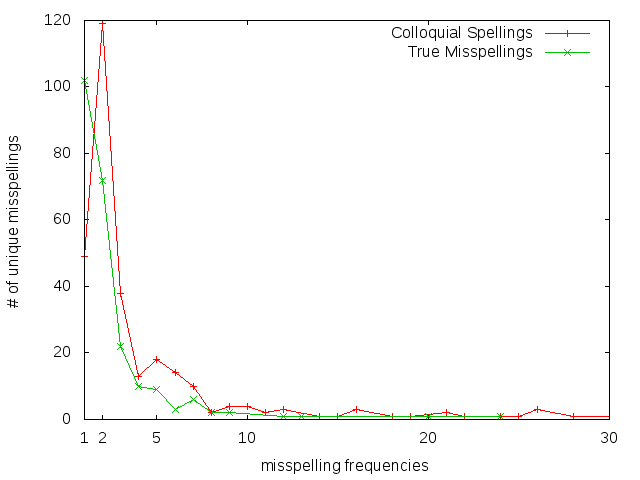
\includegraphics[width=\textwidth]{data/img/hunspell_spell.png}
    \label{fig:misspl-hunspell}
  \end{minipage}
  \hspace{0.5cm}
  \begin{minipage}[b]{0.45\linewidth}
    \caption{Frequency distributions of non-standard spellings in data
      analyzed with \texttt{TreeTagger}}
    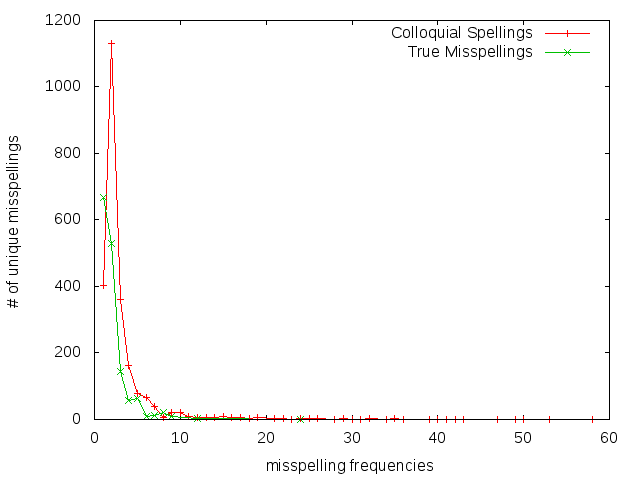
\includegraphics[width=\textwidth]{data/img/treetagger_spell.png}
    \label{fig:misspl-ttagger}
  \end{minipage}
\end{figure}

As can be seen from the figures, both kinds of spelling variations
have nearly Zipfian distribution. However colloquial spelling
variants, if used, tend to be used frequently whereas non-colloquial
misspellings are rather represented by sporadic singletons. This could
be explained by the fact that colloquial spellings are usually formed
by systematic rewriting processes which are also normally applied to
frequently used words. True misspellings, on the contrary, are rather
produced by occasional slips of the finger, so they neither have an
apparent system in them nor they tend to reoccur in text.

On closer examination of colloquial spellings, it could be found that
a large part of them was a result of phonetically motivated
rewritings.

According to our data, the most productive of such slang producing
processes turned out to be:
\begin{itemize}
  \item Omission of `e' in unstressed positions, e.g. \textit{w\"urd},
    \textit{zuguckn} etc. In cases when `e' was part of the impersonal
    pronoun ``es'' following a verb, the remaining `s' of this pronoun
    was usually appended to the preceding verb form,
    e.g. \textit{wirds} instead of \textit{wird es};

  \item Complete omission or replacement of final consonants with
    their voiceless equivalents, e.g. \textit{nich} instead of
    \textit{nicht} or \textit{Tach} instead of \textit{Tag};

  \item Omissions of `ei' from indefinite articles, e.g. \textit{ne} instead
    of \textit{eine} or \textit{nem} in lieu of \textit{einem};

  \item Multiple repetions of characters as a means of expressing elongation
    of sounds, e.g. \textit{Hilfeeee}, \textit{s\"u\"u\"u\ss};
\end{itemize}

Since all of the above processes followed some specific formation
patterns. We developed a set of reverese transformation rules which
first captured tokens with suspicious character sequences, checked
them in the dictionary, and if these words were not found there, a
transformation associated with each matched incorrect character
sequence was applied.

TODO: more detailed and coherent description of rule module

Unfortunately, spelling variants which were classified as true
misspellings did not show any regularities except for cases of
incorrect spelling of sharp ``s'' and umlauts. While writting of
``ss'' instead of sharp ``s'' could also be considered as correct
variant with regard to the Swiss norm. For umlauts, a straightforward
replacement of character sequences like ``ae'', ``oe'' or ``ue''
because these character sequences also appeared in regular German
words like ``israelisch'' or ``quer''. Therefore a set of exceptional
cases had to be found before applying substitutions. As a possible
source of such exceptions we considered words classified by us as
in-vocabulary or valid out-of-vocabulary terms. Another source of
possible exceptions was a corpus of newspaper texts which by
definition were supposed to contain only proof-read content. To derive
exceptional character sequences, we subsequently expanded the
substrings to the left and to the right or simultaneously to both
directions until these subsequence only captured words present in our
``normal'' data without capturing any misspeling from the list. After
having collected exceptions, we only applied replacement operation to
text spans lying in between exceptional substrings. On another test
set of 500 cases, this method turned out to have made only one
mistake. It replaced the word ``zuende'' with ``z\"unde'' in the
sentence ``RT @Netznarr: Als Amtstr\"ager wei\ss man, dass es zuende
geht, wenn man in Umfragen unbeliebter als Westerwelle ist. \#Wulff''

TODO: should be described as algorithm, should the same approach be
tried for other misspelling char sequences?


%
\section{Evaluation}\label{evaluation}
To evaluate our system, we first performed an intrinsic evaluation by
measuring the rate by which the amount of unknown tokens was reduced
for \texttt{TreeTagger} and \texttt{hunspell}.

TODO: figures for OOV rates after normalization.

To comply with metrics commonly used for evaluating text normalization
procedures for other languages, we also measured word error rate (WER)
and sentence error rate (SER) for restoration of non-standard and
incorrect spellings.

TODO: WER and SER figures after normalization.

Finally, as a first step towards an extrinsic evaluation, we measured
how \texttt{TreeTagger} performance changed after normalization step
was applied

TODO: Figures for tagging quality before and after normalization.


\section{Conclusions and Future Work}\label{conclusion}

With this article, we hope to have provided a better insight into the
nature and composition of ill-formed words in German Twitter
messages. As was shown in Section \ref{error:analysis}, special markup
elements and casual sppellings account for more than a half unknown
words discovered in Tweets. Furthermore, almost three quarters of
non-standard spellings could be regarded as colloquial spelling
variants rather than occasional slip of the finger. Such colloquial
spellings also showed the tendency to be formed by well formalized
processes and to be used over and over again in texts.

We also suggested a rule-based text normalization approach which could
serve as a baseline comparison measure for future normalization
methods which may be suggested for German tweets. As was shown in
previous sections, our approach could effectively address some ofthe
most frequent phenomena which contribute to a higher rate of
out-of-vocabulary words in Twitter texts such as Twitter-specific
elements and non-standard spellings.

We are going to make our classification and test data available online
at \url{http://dasom.ling.uni-potsdam.de/} under the terms consistent
with Twitter regulations. Our classified data could, in our opinion,
significantly save tedious manual work for other researchers.

Admittedly, our method still could be further refined and improved. As
possible steps for such refinement, we see a possible addition of a
machine-learning classifier which could help distinguish spelling
mistakes from valid unknown words. On the other side, a better
disambiguation of suggested replacement variants for misspellings
could be achieved by letting part-of-speech tagger process a word grid
with input tokens and their suggested replacements. At the end of
tagging, not only the most probable tag sequence but the most likely
word/tag mesh could be chosen in a single run. At any rate, these
steps are beyond the scope of this work. But we hope to have laid the
groundwork for them.

\subsection*{\ackname}

This work was financially supported by ... as part of collaborative
project ``...''. The authors are also thankful to ... for help with
the analysis of data.

%
% ---- Bibliography ----
%
\bibliographystyle{splncs}
\begin{thebibliography}{}
\bibitem[2006]{aw}
  Aw, A., Zhang, M., Xiao, J., Su, J.: %
  A Phrase-based Statistical Model for {SMS} Text Normalization. %
  COLING/ACL (2006) 33--40 %

\bibitem[2002]{bangalore}
  Bangalore, S., Murdock, V., Riccardi, G.: %
  Bootstrapping Bilingual Data using Consensus Translation for a %
  Multilingual Instant Messaging System. %
  COLING (2002) 33--40 %

\bibitem [2010]{beaufort}
  Beaufort, R., Roekhaut, S., Cougnon, L. A.,  Fairon, C.: %
  A Hybrid Rule/Model-Based Finite-State Framework for %
  Normalizing SMS Messages. %
  ACL (2010) 770--779 %

\bibitem[2000]{brill}
  Brill, E., Moore, R. C.: %
  An improved model for noisy channel spelling correction. %
  ACL %
  (2000) 286--293 %

\bibitem[2003]{alexander-clark}
  Clark, A.: %
  Pre-processing very noisy text. %
  In Proceedings of Workshop on Shallow Processing of Large Corpora. %
  (2003) 12--22

\bibitem[2007]{choudhury}
  Choudhury, M., Saraf, R., Jain, V., Mukherjee, A., Sarkar, S., Basu %
  A.: %
  Investigation and Modeling of the Structure of Texting Language. %
  International Journal of Document Analysis and Retrieval: Special %
  Issue on Analytics of Noisy Text. {\bfseries 10} %
  (2007) 157--174 %

\bibitem[1991]{church}
  Church, K., Gale, W.: %
  Probability scoring for spelling correction. %
  Statistics and Computing. {\bfseries 1} %
  (1991) 93--103 %

\bibitem[2003]{clark}
  Clark, A.,: %
  Pre-Processing very noisy text. %
  In Proceedings of Workshop on Shallow Processing of Large Corpora. %
  Corpus Linguistics. %
  Lancaster (2003)

\bibitem[2011]{clark-araki}
  Clark, E., Araki, K.: %
  Text Normalization in Social Media: Progress, Problems and %
  Applications for a Pre-processing System of Casual English. %
  PACLING. Procedia - Social and Behavioral Sciences {\bfseries 27} %
  (2011) 2--11

\bibitem[2009]{cook}
  Cook, P., Stevenson, S.: %
  An unsupervised model for text message normalization, %
  Proceedings of the Workshop on Computational Approaches %
  to Linguistic Creativity. %
  CALC '09. (2009) 71--78

\bibitem[2006]{dorsey}
  Dorsey, J.: %
  "just setting up my twttr". %
  \url{https://twitter.com/jack/status/20} %
  Accessed February 26, 2013. (2006)

\bibitem[2011]{han}
  Han, B., Baldwin, T.: %
  Lexical Normalization of Short Text Messages: Makn Sens %
  a \#{}twitter. %
  ACL HLT. %
  (2011) 368--378

\bibitem[2008]{jurafsky}
  Jurafsky, D., Martin, J. H.: %
  Speech and Language Processing. 2nd Edition. %
  Prentice Hall (2008) 129, 323

\bibitem [2010]{kaufmann}
  Kaufmann, M.: %
  Syntactic normalization of twitter messages. %
  The 8-th International Conference on Natural Language Processing. %
  (2010)

\bibitem [2008]{kobus}
  Kobus, C., Yvon, F., Damnati, G.: %
  Normalizing {SMS}: are Two Metaphors Better than One? %
  COLING (2008) 441--448

\bibitem[1992]{kukich}
  Kukich, K.: %
  Techniques for Automatically Correcting Words in Text. %
  ACM Computing Surveys {\bfseries 24/4} (1992) 378--439

\bibitem[1991]{mayes}
  Mayes, E., F. Damerau, et al.: %
  Context Based Spelling Correction. %
  Information Processing and Management. 27(5) %
  (1991) 517--522

\bibitem[2012]{guardian:sms}
  McVeigh, T.: %
  Text messaging turns 20. %
  The Observer (December 1, 2012)

\bibitem[2012]{mukherjee}
  Mukherjee, S., Malu, A., Balamurali, A. R., Bhattacharyya, P.: %
  TwiSent: A Multistage System for Analyzing Sentiment in Twitter. %
  In Proceedings of The 21st ACM Conference on Information and %
  Knowledge Management CIKM 2012, Hawai, (Oct 29 - Nov 2, 2012)

\bibitem [2013]{oliva}
  Oliva, J., Serrano, J. I., and Del Castillo, M. D., %
  and Igesias, �.: %
  A {SMS} normalization system integrating multiple %
  grammatical resources. %
  Natural Language Engineering. %
  (2013) 121--141 %

\bibitem [2002]{papineni}
  Papineni, K., Roukos, S., Ward, T., Zhu, W.-J.: %
  Bleu: a Method for Automatic Evaluation of Machine Translation. %
  ACL (2002) 311--318

\bibitem [2011]{parker}
  Parker, A.: %
  Twitter's Secret Handshake. %
  The New York Times, Page ST1, (June 10, 2011)

\bibitem [1980]{petersen}
  Petersen, L. J.: %
  Computer Programs for Detecting and Correcting Spelling Errors. %
  Communications of the ACM {\bfseries 23/ 12} (1980) 676--687

\bibitem[2012]{nyt:pope}
  Pianigiani, G., Donadio, R.: %
  Twitter Has A New User: The Pope. %
  The New York Times. Page A6. (December 4, 2012)

\bibitem[2001]{sproat}
  Sproat, R., Black, A. W., Chen, S. F., Kumar, S., %
  Ostendorf, M., Richards, Ch.: %
  Normalization of non-standard words. %
  Computer Speech \& Language, {\bfseries 15/3} (2001) 287--333

\bibitem[1994]{schmid}
  Schmid, H.: %
  Probabilistic Part-of-Speech Tagging Using Decision Trees. %
  In Proceedings of International Conference on New Methods in %
  Language Processing. (1994)

\bibitem[1948]{shannon}
  Shannon, C. E.: %
  A mathematical theory of communication. %
  Bell system techical journal, 27:379--423 %
  (1948) 623--656

\bibitem[1996]{sparck}
  Sparck Jones, K., Galliers, J. R.: %
  Evaluating Natural Language Processing Systems. %
  An Analysis and Review. Lecture Notes in Computer %
  Science 1083, Springer. (1996)

\bibitem[2012]{terdiman}
  Terdiman, D.: %
  Report: Twitter hits half a billion tweets a day. %
  \url{http://timmurphy.org/2009/07/22/line-spacing-in-latex-documents/},%
  Accessed February 26, 2013. (2012)

\bibitem[2002]{toutanova}
  Toutanova, K., Moore, R. C.: %
  Pronunciation Modeling for Improved Spelling Correction. %
  ACL (2002) 144--151

\end{thebibliography}
%
% ---- End of Bibliography ----
%
\end{document}
